\documentclass[10pt,a4paper]{article}
\usepackage[utf8]{inputenc}
\usepackage[english]{babel}
\usepackage[left=2cm,right=2cm,top=2cm,bottom=2cm]{geometry}
\usepackage{setspace}
\usepackage{parskip}
\usepackage{amsmath}
\usepackage{amsfonts}
\usepackage{amssymb}
\usepackage{graphicx} 
\usepackage{hyperref}
\usepackage{apacite} % APA citation
\usepackage{floatrow} % Always centers pictures
\usepackage{listings}
\usepackage{graphicx}
\lstset{breaklines=true, frame=L}


\author{Gasper Trebse}
\title{Monetary Economics 2\\
\textbf{Theoretical Assignment} \\
Monetary economy with pandemic and fiscal transfer function}
\date{\today}


\begin{document}
\doublespacing
\pagenumbering{gobble}% Remove page numbers (and reset to 1)
\clearpage
\thispagestyle{empty}
\maketitle
\clearpage
\singlespacing
\pagenumbering{roman}% Roman page numbers (and reset to 1)
\tableofcontents 
\bigskip
\listoffigures
\clearpage
\pagenumbering{arabic}% Roman page numbers (and reset to 1)
\doublespacing

\section{Introduction}
This theoretical assignment explores a New Keynesian dynamic stochastic general equilibrium (DSGE) model with price rigidity. The DSGE is an RBC model with nominal sticky prices. In this case, the model introduces Calvo staggered prices. The model is comprised of three types of entities: Firms, government and households. The households maximize their utility by choosing between their consumption, labor, and investments. Firms are divided into final goods producers and intermediate goods producers. The intermediate goods producers compete on a monopolistically competitive market and set their prices according to the Calvo specification. Final goods producers buy intermediate goods from the intermediate goods producers in order to fill a unit "basket" of goods. To produce the goods firms employ capital and labor and they distribute the the profits to households. The government collects lump-sum taxes from households and uses it to finance their spending.\\
In the following sections the model equations are derived. These include the optimization problems of firms and households. These equations are log-linearized in the next section. The last section focuses on simulating the model in Dynare and provides evaluation of the simulation outputs.


\section{Description of the model}
\subsection{Households}
The representative households choose 
$\left\lbrace C_{t+i}, N_{t+i}, \frac{M_{t+i}}{P_{t+i}}, \frac{B_{t+i}}{P_{t+i}} \right\rbrace ^{\infty} _{i=1}$
to maximize their infinite forward looking stream of utilities defined by the equation:
\begin{equation}\label{eq:1}
 E_{t} \sum^{\infty}_{t=0} \beta^{i} \left[
\dfrac{\chi_{t}}{1-\gamma} C^{1-\gamma}_{t+i}
+ 
\dfrac{a_{m}}{1-\gamma_{m}} \left(\dfrac{M_{t+i}}{P_{t+i}}\right)^{1-\gamma_{m}}
-
\dfrac{a_{n}}{1+\gamma_{n}} N_{t+i}^{1+\gamma_{n}}
\right]
\end{equation}

subject to the real budget constraint:

\begin{equation}\label{eq:2}
C_{t} = \dfrac{W_{t}}{P_{t}}N_{t} + \Pi_{t} -T_{t} 
- \dfrac{M_{t}-M_{t-1}}{P_{t}}
- \dfrac{Q_{t} B_{t}- B_{t-1}}{P_{t}}
\end{equation}


where $\gamma, \gamma_{m} < 1 $ and $\gamma_{n} > 1$ and
$B_{t}$ is one-period risk-free bond, purchased at the beginning of period $t$ that pay the net interest rate $i$ at the end of period $t$. $\chi_{t}$ are consumer confidence shocks, which follow an AR(1) process. $W_{t}$ is the economy-wide nominal wage, $\Pi_{t}$ are profits distributed to households from firms they own, and $T_{t}$ are lump-sum taxes levied on the households by the government. \\

The FOC for the household optimization process will be derived using the Bellman equation \eqref{eq:bellman}
\begin{equation}\label{eq:bellman}
v \left( \dfrac{M_{t-1}}{P_{t}}, \dfrac{B_{t-1}}{P_{t}} \right)
= \max_{N_{t}, \frac{B_{t}}{P_{t}}, \frac{M_{t}}{P_{t}}}
\left[
\dfrac{\chi_{t}}{1-\gamma} C^{1-\gamma}_{t+i}
+ 
\dfrac{a_{m}}{1-\gamma_{m}} \left(\dfrac{M_{t+i}}{P_{t+i}}\right)^{1-\gamma_{m}}
-
\dfrac{a_{n}}{1+\gamma_{n}} N_{t+i}^{1+\gamma_{n}}
\\
+ 
\beta E_{t} v \left( \dfrac{M_{t}}{P_{t+1}}, \dfrac{B_{t}}{P_{t+1}} \right) \right]
\end{equation}
subject to \eqref{eq:2}.
\subsection{FOC w.r.t labor (N)}
To calculate the implicit labor-supply function we partially derive the bellman equation \eqref{eq:bellman} with respect to N.
\begin{equation}
\frac{\partial v \left( \dfrac{M_{t-1}}{P_{t}}, \dfrac{B_{t-1}}{P_{t}} \right)}{\partial N_t} =
\frac{\partial \left(\frac{\chi_{t}}{1-\gamma} C^{1-\gamma}\right)}
{\partial N_{t}}
-
\frac{\partial \left( 
\frac{a_{n}}{1-\gamma^{n}} N_{t}^{1+\gamma_{n}} \right)}
{\partial N_{t}}
= 0 \end{equation}
\begin{equation}
\frac{\partial \left(\frac{\chi_{t}}{1-\gamma} C^{1-\gamma}\right)}
{\partial N_{t}} \cdot \dfrac{\partial C_{t}}{\partial N_{t}}
-
\dfrac{a_{n}}{1+\gamma_{n}}(1+\gamma_{n})N_{t}^{\gamma_{n}}
= 0 
\end{equation}
\begin{equation}
\dfrac{\chi_{t}(1-\gamma)}{(1-\gamma)} C_{t}^{-\gamma} \dfrac{W_{t}}{P_{t}}
- a_{n} N_{t}^{\gamma_{n}}
= 0 \end{equation}
Reordering and simplifying the equation above gives us the implicit labor supply function \eqref{eq:implicitLabor}:

\begin{equation}\label{eq:implicitLabor} 
\dfrac{W_{t}}{P_{t}} 
= 
a_{n} \dfrac{N_{t}^{\gamma_{n}}}{\chi_{t} C_{t}^{-\gamma}}
\end{equation}

The implicit labor supply function gives us a relation between the marginal rate of substitution between work and consumption of households. In equilibrium the marginal rate of substitution between leisure and consumption (RHS) must be equal to nominal wage (LHS). The consumer confidence shock defined by $\chi_{t}$ is inversely correlated with wage, which forces the wage to drop in case of a positive shock and rise in case of a negative shock.
\subsection{FOC w.r.t bonds $(B_{t}/P_{t})$}
The intertemporal optimization for bonds is calculated by taking the derivative of \eqref{eq:bellman} with respect to $(B_{t}/P_{t})$.
$$\chi_t C_t^{-\gamma} Q_{t} + \beta E_{t} \left( v_{\frac{B_t}{P_{t+1}}} \left(  \frac{M_t}{P_{t+1}}, \frac{B_t}{P_{t+1}}\right) \frac{\partial \frac{B_t}{P_{t+1}}}{\partial (\frac{B_t}{P_t})} \right)=0 $$

where:
$$ \frac{P_t}{P_{t+1}}= \frac{\partial \frac{B_t}{P_{t+1}}}{\partial \frac{B_t}{P_t}} $$

resulting in:
\begin{equation}\label{eq:8}
\chi_t C_t^{-\gamma} Q_{t} + \beta E_{t} \left( v_{\frac{B_t}{P_{t+1}}} \left(  \frac{M_t}{P_{t+1}}, \frac{B_t}{P_{t+1}}\right) \frac{P_{t}}{P_{t+1}} \right)=0
\end{equation}

To derive the second part of the equation we shift the Bellman equation for one period and partially deriving by $(B_{t}/P_{t+1})$:
$$v_{\frac{B_t}{P_{t+1}}} \left(  \frac{M_t}{P_{t+1}}, \frac{B_t}{P_{t+1}}\right)=\chi_{t+1} C_{t+1}^{-\gamma} \left( 1 - Q_{t} \frac{\partial \frac{B_{t+1}}{P_{t+2}}}{\partial \frac{B_t}{P_{t+1}}}\right)  + \beta E_{t+1} v_{\frac{B_{t+1}}{P_{t+2}}} \frac{\partial \frac{B_{t+1}}{P_{t+2}}}{\partial \frac{B_t}{P_{t+1}}} $$\\
which simplifies to
\begin{equation}
v_{\frac{B_t}{P_{t+1}}} \left(  \frac{M_t}{P_{t+1}}, \frac{B_t}{P_{t+1}}\right)=\chi_{t+1} C_{t+1}^{-\gamma}
+ 
\underbrace{
\left( -\chi_{t+1} C_{t+1}^{-\gamma}Q_{t}\frac{P_{t+2}}{P_{t+1}}+ \beta v_{\frac{B_{t+1}}{P_{t+1}}} \right)
}_{\text{envelope theorem, shift \eqref{eq:8} by 1 forward}}
\frac{\partial \frac{B_{t+1}}{P_{t+2}}}{\partial \frac{B_t}{P_{t+1}}}
\end{equation}
By using the envelope theorem we can shift the \eqref{eq:8} by one time period forward which simplifies to:
\begin{equation}
v_{\frac{b_{t}}{P_{t+1}}} = \chi_{t+1}C_{t+1}^{-\gamma}
\end{equation}\label{eq:10}
By using \eqref{eq:8} and \eqref{eq:10} we get the Euler equation
\begin{equation}
C_t^{-\gamma}= \beta \frac{1}{Q_{t}} \frac{P_{t}}{P_{t+1}} C_{t+1}^{-\gamma}\frac{\chi_{t+1}}{\chi_t}
\end{equation}
\begin{equation}\label{eq:euler} 
C_t^{-\gamma}= \beta R_{t+1} C_{t+1}^{-\gamma}\frac{\chi_{t+1}}{\chi_t}
\end{equation}
where R is the real rate of return that corrects for inflation
$$R_{t+1} = \frac{(1+i_t) P_t}{P_{t+1}}$$.
From the euler equation \eqref{eq:euler} we can conclude that the current consumption $C_{t}$ is determined by the discounted future consumption $C_{t+1}$, the real rate of return and the ratio of current and future consumer shock. An increase in the consumer shock in the next period would rise the current consumption while a decrease to the shock in the future period would increase the instantaneous consumption.

\subsection{FOC w.r.t money $(M_{t}/P_{t})$}
The FOC derivation begins with taking a partial derivative of the Bellman equation \eqref{eq:bellman} w.r.t $\frac{M_{t}}{P_{t}}$ which gives us:
\begin{equation*}
\chi_{t}C_{t}^{-\gamma}\frac{\partial C_{t}}{\partial \frac{M_{t}}{P_{t}}} + a_{m}(\frac{M_{t}}{P_{t}})^{1-\gamma_{m}}+ \beta E_{t}( v_{(\frac{M_{t}}{P_{t+1}})}(\frac{M_{t}}{P_{t+1}},\frac{B_{t}}{P_{t+1}})\frac{P_{t}}{P_{t+1}})=0
\end{equation*}
or
\begin{equation}\label{eq:13}
-\chi_{t}C_{t}^{-\gamma} + a_{m}(\frac{M_{t}}{P_{t}})^{1-\gamma_{m}}+ \beta E_{t}( v_{(\frac{M_{t}}{P_{t+1}})}(\frac{M_{t}}{P_{t+1}},\frac{B_{t}}{P_{t+1}})\frac{P_{t}}{P_{t+1}})=0
\end{equation}

by shifting the Bellman equation one period forward and taking the derivative w.r.t $M_{t}/P_{t+1}$ we get:
\begin{equation}\label{eq:14}
\chi_{t+1}C_{t+1}+\underbrace{\left(-\chi_{t+1}C_{t+1}^{-\gamma}\frac{P_{t+2}}{P_{t+1}}+a_m\left(\frac{M_{t+1}}{P_{t+1}}\right)^{-\gamma_m}\frac{P_{t+2}}{P_{t+1}}+\beta E_{t+1}v_{\frac{M_{t+1}}{P_{t+2}}}\right)}_{\text{envelope theorem, shift \eqref{eq:13} by 1 forward}}\frac{\frac{\partial M_{t+1}}{P_{t+2}}}{\frac{\partial M_{t}}{P_{t+1}}}=0
\end{equation}
Which results in
\begin{equation*}
v_{\frac{M_{t}}{B_{t+1}}} = \chi_{t+1}C_{t+1}^{-\gamma}
\end{equation*}
Finally, we get the equation:
\begin{equation}\label{eq:eulerMoney}
a_{m}\left(\frac{M_{t}}{P_{t}}\right)^{-\gamma_{m}}+\beta E_{t}\left[\chi_{t+1}C_{t+1}^{-\gamma}\frac{P_{t}}{P_{t+1}}\right]=\chi_{t}C_{t}^{-\gamma}
\end{equation}
by dividing the equation by $\chi_{t}C_{t}^{-t}$ and a bit of simplification we get to:
\begin{equation}
\Delta_{t}=\frac{i_{t}}{1+i_{t}}=a_{m}\frac{\left(\frac{M_{t}}{P_{t}}\right)^{-\gamma_{m}}}{\chi_{t}C_{t}^{-\gamma}}
\end{equation}
The equation \eqref{eq:eulerMoney} describes the relationship the opportunity cost of holding money and the marginal rate of substitution between money and consumption. A positive consumer confidence shock will decrease the money holdings and increase the contemporaneous consumption.

\subsection{Firms}
The economy consists of a continuum of perfectly competitive final goods producers with the following production function:
\begin{equation}
Y_t^f = \left[ \int_{0}^{1} Y_t^f(z)^ \frac{\varepsilon_{t}-1}{\varepsilon_{t}} dz \right]^\frac{\varepsilon_{t}}{\varepsilon_{t}-1}
\end{equation},
and a continuum of monopolistically competitive intermediate goods producers who, for the generic good z, operate the following production function
\begin{equation}
Y_{t}(z) = A_{t}N_{t}(z)
\end{equation}
Intermediate good producers set prices according to Calvo's specification. The probability for them to change prices is specified by $1-\theta$ while the probability to keep their prices at the previous level is $\theta$. The equations \eqref{eq:19},\eqref{eq:20},\eqref{eq:21} describe shocks.
\begin{equation}\label{eq:19}
\ln A_{t}=(1-\rho_{A})\ln A + \rho_{A}\ln A_{t-1} + \varepsilon_{t}^{A}
\end{equation}
\begin{equation}\label{eq:20}
\ln\chi_{t}=(1-\rho_{\chi})\ln \chi + \rho_{\chi}\ln \chi_{t-1} + \varepsilon_{t}^{\chi}
\end{equation}
\begin{equation}\label{eq:21}
\ln\varepsilon_{t}=(1-\rho_{\epsilon})\ln\epsilon + \rho_{\epsilon}\ln \epsilon_{t-1} + \epsilon_{t}
\end{equation}
\subsection{Final good producers}
The final goods producers will minimize their costs by choosing $Y_{t}^{f}(z)$ while still filling up the full basket of goods. The problem is described in the following equations:
\begin{equation}
min \int_0^1 Y_t^f(z) P_t(z) dz
\end{equation}
subject to
\begin{equation}
\left[ \int_{0}^{1} Y_t^f(z)^ \frac{\varepsilon_{t}-1}{\varepsilon_{t}} dz \right]^\frac{\varepsilon_{t}}{\varepsilon_{t}-1}\geqslant \bar{Y}
\end{equation}
The minimization problem will be solved using the lagrangian:
\begin{equation}
\mathcal{L} = \int_0^1 Y_t^f(z) P_t(z) dz - \lambda \left \{ \left[ \int_{0}^{1} Y_t^f(z)^ \frac{\varepsilon_{t}-1}{\varepsilon_{t}} dz \right]^\frac{\varepsilon_{t}}{\varepsilon_{t}-1} - \bar{Y}\right\}
\end{equation}
The FOC wrt $Y_{t}^{f}(z)$:
gives us:
\begin{equation}\label{eq:25}
0=\int_{0}^{1}P_{t}(z)dz - \lambda(\left[\int_{0}^{1}Y_{t}^{f}(z)^{\frac{\varepsilon_{t}-1}{\epsilon_{t}}}\right]^{\frac{\epsilon_{t}}{\epsilon_{t}-1}}Y_{t}^{f}(z)^{-\frac{1}{\epsilon_{t}}}
\end{equation}\label{eq:26}
By inserting the original production fuction in \eqref{eq:25} we get
\begin{equation}
P_t(z)= \lambda \left( \frac{Y_t^f(z)}{Y_t^f}\right)^{-\frac{1}{\varepsilon_{t}}}
\end{equation}
By multiplying by $\int_{0}^{1}\frac{Y_{t}^{f}(z)}{Y_{t}}^{-\frac{1}{\varepsilon_{t}}}dz$ we get:
\begin{equation}
\frac{1}{Y_t^f} \underbrace{\int_{0}^{1} P_t(z)Y_t^f (z)dz}_{\text{=E(total cost)}} =
\lambda 
\underbrace{
\int_0^1 \left( \frac{Y_t^f(z)}{Y_t^f} \right)^{-\frac{1}{\varepsilon}} \frac{Y_t^f(z)}{Y_t^f} dz
}_{=1}
\end{equation}
By simplifying we get:
\begin{equation}
\frac{E_{t}^{f}}{Y_{t}^{f}} = \lambda \Rightarrow E_{t}^{f}=\lambda Y_{t}^{f}
\end{equation}
For competitive final goods $E_{t}^{f}=P_{t}^{f}Y_{t}^{f}$ holds which leads to:
\begin{equation}\label{eq:29}
\lambda = P_{t}
\end{equation}
By using \eqref{eq:29} and \eqref{eq:26} we get
\begin{equation}\label{eq:30}
P{t}(z)=P_{t}(\frac{Y_{t}^{f}(z)}{Y_{t}^{f}})^{-\frac{1}{\varepsilon_{t}}} \Leftrightarrow Y{t}(z)=Y_{t}(\frac{P_{t}^{f}(z)}{P_{t}^{f}})^{-\epsilon_{t}}
\end{equation}
The equations \eqref{eq:30} gives us optimal relation between the amount of each variety of prices of each variety and the total price.
\subsection{Price index}
The price index is the price of a complete basket of goods comprised out of the variety available in the economy and is equal to:
$$P_{t}=\int_{0}^{1}P_{t}(z)Y_{t}(z)dz$$ s.t. $$Y_{t}=1$$
By inserting \eqref{eq:30} we get:
\begin{equation}
P_{t}^{1-\varepsilon_{t}}=\int_{0}^{1}P_{t}(z)^{1-\epsilon_{t}}dz
\end{equation}
or
\begin{equation}\label{eq:32}
P_{t}=(\int_{0}^{1}P_{t}(z)^{1-\varepsilon_{t}}dz)^\frac{1}{1-\epsilon_{t}}
\end{equation}
\subsection{Intermediate goods producer}
A continuum of monopolistically competitive producers who for generic good z, operate to following production function
\begin{equation}
Y_{t}(z)=A_{t}N_{t}(z)
\end{equation}
The firms change prices based on the Calvo specification. They face marginal costs that follow the function:
$$ MC = \frac{\partial TC}{\partial Y}= \frac{W_t}{A_tP_t(z)} $$
The firms optimization problem involves choosing between labor employed, price, and output.
$$ \max_{P_t(z), N_t(z), Y_t(z)}
\left[
\dfrac{P_t(z)}{P_t} Y_t(z)
-
\dfrac{W_t}{P_t} N_t(z)
\right]
$$
s.t.
$$
Y_t(z)=A_tN_t(z)  \wedge  Y_t(z)=(\frac{P_t(z)}{P_t})^{-\varepsilon_t}Y_t
$$
\subsection{Optimization problem under price flexibility}
The optimization problem under price flexibility is defined by the following equation
$$ \max_{P_t(z), N_t(z), Y_t(z)}
\left[
\dfrac{P_t(z)}{P_t} Y_t(\frac{P_t(z)}{P_t)}^{-\varepsilon_t}
-
\frac{W_t}{P_t}N_t(z)
\right]
$$
which simplifies to:
$$ \max_{P_t(z), N_t(z), Y_t(z)}
\left[
((\dfrac{P_t(z)}{P_t})-\frac{W_t}{P_tA_t})(\frac{P_t(z)}{P_t})^{-\varepsilon_t}Y_t
\right]
$$
The FOC w.r.t $P_t(z)$:
$$
(1-\varepsilon_t)\frac{1}{P_t^{1-\epsilon_t}} P_t(z)^{-\epsilon_t} -
 \frac{W_t}{P_tA_t}(-\varepsilon_t)\frac{1}{P_t^{-\epsilon}} P_t(z)^{-1-\epsilon_t)}
$$
Which simplifies to:
\begin{equation}\label{eq:34}
MC_{t,t}=\frac{1}{1+\mu} \qquad \textrm{or} \qquad \frac{P_t(z)^*}{P_t} = MC_t(1+\mu)
\end{equation}

The equation \eqref{eq:34} tells us that the price is equal to the marginal costs times the mark-up which is in our case $1+\mu$
\subsection{Optimization problem under Calvo pricing}
The following equation describes the optimization under Calvo pricing:
\begin{equation}\label{eq:35}
\max_{P_{t}(z)}E_{t}\sum_{i=0}^{\infty}
\theta^{i}Q_{t,t+i}
\left[
\left(\frac{P_{t}(z)}{P_{t+i}}-\frac{W_{t+i}}{A_{t+i}P_{t+i}}
\right)
\left(\frac{P_t(z)}{P_{t+i}}
\right)^{-\varepsilon_t}Y_{t+i}
\right]
\end{equation}
The FOC w.r.t. $P_t(z)$:
\begin{equation}
E_{t}\sum_{i=0}^{\infty}
\theta^{i} Q_{t,t+i}(\frac{P_t(z)}{p_t+i})^{1-\varepsilon_t}Y_{t+i}
=
(1+\mu_t)E_t\sum_{i=0}^{\infty}\theta^iQ_{t+i}MC_{t+i}(\frac{P_t(z)}{p_t+i})^{-\varepsilon_t}Y_{t+i}
\end{equation}
Simplifying and using $MC_{t+i,t}^n=P_tMC_{t+i,t}$ and $\pi_{t,t+i}=\frac{P_{t+i}}{P_t}$ gives us:
\begin{equation}
P_t^*E_t\sum_{i=0}^{\infty}\theta^iQ_{t+i}(\frac{P_t(z)}{P_t^{1-\varepsilon_t}}) Y_{t+i}
=
(1+\mu_t)E_t\sum_{i=0}^{\infty}\theta^iQ_{t+i}\pi_{t,t+i}MC_{t+i}^n(\frac{P_t(z)}{P_t^{1-\varepsilon_t}})
\end{equation}
Finally,
\begin{equation}\label{eq:38}
P_t(z)^*=(1+\mu_t)\sum_{i=0}^{\infty}\omega_{t,t+i}\pi_{t,t+i}MC_{t+i}
\end{equation}
With the $\omega$ defined by the following equation:
\begin{equation}
\omega_{t+i} = 
\frac{
E_t \theta^i Q_t Y_t \left(\frac{1}{P_{t+i}}\right)^{1-\varepsilon_t}
}{
E_{t}\sum_{i=0}^{\infty} \theta^i Q_t Y_t \left(\frac{1}{P_{t+i}}\right)^{1-\varepsilon_t}
}
\end{equation}
The equation \eqref{eq:38} describes the relation between the price for a specific variety and the sum of weighted future marginal costs times the mark up. By ignoring the Calvo pricing the \eqref{eq:38} simplifies to the equation \eqref{eq:34}. We can see that with the new expression for the marginal cost, the optimal price depends also on the stream of future expected inflation rates.
\subsection{Equilibrium conditions}
The equilibrium conditions:
$$P_t(z)=P_t \ \ \ \ \ \forall z$$ 
$$Y_t(z)=Y_t \ \ \ \ \ \forall z$$ 
$$N_t(z)=N_t \ \ \ \ \ \forall z$$
The economy wide equilibrium condition is:
$$C_t+G_t=Y_t$$
Bonds market clearing condition:
$$B_t=0$$
\subsection{Aggregation}
The labor market clearing condition gives us the aggregate level of output function:
\begin{equation}
N_t=\int_{0}^{1}N_t(z)dz=
\int_{0}^{1}\frac{Y_t(z)}{A_t}dz=
\frac{Y_t}{A_t}\underbrace{\int_{0}^{1}\left(\frac{P_t(z)}{P_t}\right)^{-\varepsilon_t}dz
}_{\text{=Price dispersion}}
\end{equation}
The total output $Y_t$ is defined by equation:
\begin{equation}
Y_t=\frac{A_t}{\Delta_t}N_t
\end{equation}
Where $\delta$ defines the measure of price dispersion. The price dispersion forces the $Y_t$ to be too high or too low. This creates a channel for monetary policy to increase the total welfare by creating an environment with low price dispersion that allows for an optimum level of output
\section{The complete model}
The following equations describe the complete model that was derived in the previous sections:
\begin{itemize}
\item Labor market equilibrium:
\begin{equation}\label{eq:labor}
A_t= (1+\mu_t)a_n \frac{N_t^{\gamma_n}}{\chi_t C_t^{-\gamma}}
\end{equation}
\item Euler equation for bonds:
\begin{equation}\label{eq:bonds}
C_t^{-\gamma}= E_t \left[ \frac{P_t}{P_{t+1}} \frac{1}{Q_t} \frac{\chi_{t+1}}{\chi_t} \beta C_{t+1}^{-\gamma}\right]
\end{equation}
\item Euler equation for money:
\begin{equation}\label{eq:money}
\frac{M_t}{P_t}=\left(
\chi_{t} C_t^{-\gamma} \Delta_t a_m^{-1} \right)^{\frac{1}{\gamma_m}}
\end{equation}
\end{itemize}
\subsection{IS Curve}
From the Euler equation for bonds we can calculate the IS curve:
$$(Y_t-G_t)^{-\gamma}= E_t \left[
\frac{P_t}{P_{t+1}} \frac{1}{Q_t} \frac{\chi_{t+1}}{\chi_t} \beta (Y_{t+1}-G_{t+1})^{-\gamma} \right]$$
or
$$Y_t= E_t \left[
\frac{P_t}{P_{t+1}} \frac{1}{Q_t} \frac{\chi_{t+1}}{\chi_t} \beta (Y_{t+1}-G_{t+1})^{-\gamma} \right]^{-\frac{1}{\gamma}}+G_t$$
\subsection{LM curve}
From the Euler equation for money we calculate the LM curve:
$$\frac{M_t}{P_t}=\left(
\chi_{t} (Y_t-G_t)^{-\gamma} \Delta_t a_m^{-1} \right)^{\frac{1}{\gamma_m}} $$
\subsection{AS curve}
The labor market clearing equilibrium function combined with the production function leads to:
\begin{equation*}
A_t= (1+\mu_t)a_n \left(\frac{Y_t}{A_t}\right)^{\gamma_n}\frac{1}{\chi_t (Y_t-G_t)^{-\gamma}}
\end{equation*}
We can express the output $Y_t$
\begin{equation}
Y_t=\left(
a_nA_t^{-(1+\gamma_n)}(1+\mu_t)\chi_t^{-1}(Y_t-G_t)^{\gamma}
\right)^{-\frac{1}{\gamma_n}}
\end{equation}
\subsection{Stationary steady state}
The steady state of the model is defined by the following equations and conditions:
\begin{itemize}
\item The mark-up: $1+\mu$
\item The Marginal cost: $MC=\frac{1}{1+\mu}$
\item Inflation: $\frac{P_t}{P_{t+1}}=1$
\end{itemize}
From the IS curve we get:
$$ 1+i=\frac{1}{\beta} $$
The steady state level of output is defined from the AS curve:
\begin{equation}\label{eq:48}
Y_t=\left(
a_nA^{-(1+\gamma_n)}(1+\mu_t)(Y-G)^{\gamma}
\right)^{-\frac{1}{\gamma_n}}
\end{equation}
\section{Log-linearization}
Log-linearization is used in economics to express a variable in terms of a percentage deviation from a reference value. In most cases the reference value taken is the steady-state of the model that is being analyzed. Additionally, the log-linearization presents the key model equations in a simple, easily understandable manner, which is useful when presenting key findings to a general public. In the following sections the log-linearized variables will be denoted by $\hat{x_t}$.
\subsection{Resource constraint}
To aid the further log-linearizations we will first log-linearize the aggregate resource constraint
$$ C_t = Y_t + G_t $$
$$ d\ln(Y_t) = d\ln(C_t+G_t) $$
$$ d\ln(Y_t) = \frac{1}{G+C}(dC_t + dG_t)$$
$$ \hat{y_t} = \frac{1}{Y}(C\frac{dC_t}{C}+D\frac{dD_t}{D})$$
$$ \hat{y_t} = \frac{C}{Y}\hat{c_t}+\frac{G}{Y}\hat{g_t}$$
or
$$ \hat{c_t} = \frac{Y}{C}\hat{y_t}-\frac{G}{C}\hat{g_t}$$
\subsection{IS curve}
We the log-linearization process start by taking the original IS curve \eqref{eq:bonds} and taking a log of it.
$$C_t^{-\gamma}= E_t \left[ \frac{P_t}{P_{t+1}} \frac{1}{Q_t} \frac{\chi_{t+1}}{\chi_t} \beta C_{t+1}^{-\gamma}\right]$$
$$-\gamma lnC_{t}=ln\beta+lnE_{t}\left[\frac{\chi_{t+1}}{\chi_{t}}C_{t+1}^{-\gamma}(1+i_{t})\frac{P_{t}}{P_{t+1}}\right]$$
$$-\gamma lnC_{t}\approx lnE_{t}\left[\frac{\chi_{t+1}}{\chi_{t}}C_{t+1}^{-\gamma}(1+i_{t})\frac{P_{t}}{P_{t+1}}\right]$$
$$-\gamma ln C_{t} \approx d\ln(1+i_t) + E_t d \ln \frac{P_t}{P_{t+1}} -\gamma E_t d \ln C_{t+1} + E_t (\hat{\chi_{t+1}} - \hat{\chi_t)}$$
$$-\gamma\hat{c_t} = \hat{i_t} - E_{t} \hat{\pi_{t+1}} -\gamma E_t \hat{y_{t+1}}$$
$$-\gamma\ \frac{Y}{C}\hat{y_t} - \frac{G}{C} \hat{g_t}= \hat{i_t} - E_{t} \hat{\pi_{t+1}} -\gamma E_t (\frac{Y}{C}\hat{y_{t+1}} - \frac{G}{C} \hat{g_{t+1}}) + (\hat{\chi_{t+1}} - \hat{\chi_t)}$$
By using the Fisher parity $\hat{r}_{t}=\hat{i}_{t}-E_{t}\hat{\pi}_{t+1}$ and simplifying we get:
\begin{equation}\label{eq:ISloglin}
\hat{y}=E_{t}\hat{y}_{t+1}-\frac{G}{Y}E_{t}(\hat{g_{t+1}-\hat{g_t}})-\frac{C}{Y}\frac{1}{\gamma}\left(\hat{r}_{t}+E_{t}(\hat{\chi_{t+1}} - \hat{\chi_t)})\right)
\end{equation}
\subsection{Marginal cost, without nominal price rigidity}
Taking a log of \eqref{eq:implicitLabor}:
$$A_{t}MC_{t}=a_{n}\frac{\left(\frac{Y_{t}}{A_{t}}\right)^{\gamma_{n}}}{\chi_{t} C_{t}^{-\gamma}}$$
$$MC_{t}=a_{n}Y_{t}^{\gamma_{n}}A_{t}^{-\left(1+\gamma_{n}\right)}C_{t}^{\gamma}\chi_{t}^{-1}$$
$$ln{MC}_{t}=ln a_{n} + \gamma_{n}ln {Y}_{t}-\left(1+\gamma_{n}\right)ln {A}_{t}- ln \chi_{t} + \gamma ln C_{t}$$
$$\hat{mc}_{t}=\gamma_{n}\hat{y}_{t}-\left(1+\gamma_{n}\right)\hat{a}_{t}+\gamma\hat{c}_{t}-\hat{\chi_{t}}$$
In terms of consumption:
$$C_{t}=Y_{t}-G_{t}$$
$$\hat{c}_{t}=\frac{Y}{C}\hat{y}_{t}-\frac{G}{C}\hat{g}_{t}$$
$$ \hat{mc}_{t}=\hat{y}_{t}\left(\gamma_{n}+\gamma\frac{Y}{C}\right)-\left(1+\gamma_{n}\right)\hat{a}_{t}-\gamma\frac{G}{C}\hat{g}_{t}-\hat{\chi_{t}}$$
$$ln{MC}_{t}=\gamma_{n}ln {Y}_{t}-\left(1+\gamma_{n}\right)ln {A}_{t}- ln \chi_{t} + \gamma ln Y_{t} +  \gamma ln G_{t}$$
\begin{equation}\label{realMClin_old} 
\hat{mc}_{t}=\hat{y}_{t}\left(\gamma_{n}+\gamma\frac{Y}{C}\right)-\left(1+\gamma_{n}\right)\hat{a}_{t}+\gamma\frac{G}{C}\hat{g}_{t}-\hat{\chi_{t}}
\end{equation}
\subsection{Marginal cost, with nominal price rigidity}
Taking a log of \eqref{eq:implicitLabor}:
$$MC_{t}A_{t}\frac{P_t(z)}{P_t}=a_{n}\frac{\left(\frac{Y_{t}}{A_{t}}\right)^{\gamma_{n}}}{\chi_{t} C_{t}^{-\gamma}}$$
$$MC_{t}\frac{P_t(z)}{P_t}=a_{n}Y_{t}^{\gamma_{n}}A_{t}^{-\left(1+\gamma_{n}\right)}C_{t}^{\gamma}\chi_{t}^{-1}$$
$$ln{MC}_{t}+lnP_t(z)-lnP_t=ln a_{n} + \gamma_{n}ln {Y}_{t}-\left(1+\gamma_{n}\right)ln {A}_{t}- ln \chi_{t} + \gamma ln C_{t}$$
$$\hat{mc}_{t}=\gamma_{n}\hat{y}_{t}-\left(1+\gamma_{n}\right)\hat{a}_{t}+\gamma\hat{c}_{t}-\hat{\chi_{t}}-\hat{p_t^*}+\hat{p_t}$$
In terms of consumption:
$$C_{t}=Y_{t}-G_{t}$$
$$\hat{c}_{t}=\frac{Y}{C}\hat{y}_{t}-\frac{G}{C}\hat{g}_{t}$$
$$ \hat{mc}_{t}=\hat{y}_{t}\left(\gamma_{n}+\gamma\frac{Y}{C}\right)-\left(1+\gamma_{n}\right)\hat{a}_{t}-\gamma\frac{G}{C}\hat{g}_{t}-\hat{\chi_{t}}-\hat{p_t^*}+\hat{p_t}$$
$$ln{MC}_{t}=\gamma_{n}ln {Y}_{t}-\left(1+\gamma_{n}\right)ln {A}_{t}- ln \chi_{t} + \gamma ln Y_{t} +  \gamma ln G_{t}-\hat{p_t^*}+\hat{p_t}$$
\begin{equation}\label{realMClin_new} 
\hat{mc(z)}_{t}=\hat{y}_{t}\left(\gamma_{n}+\gamma\frac{Y}{C}\right)-\left(1+\gamma_{n}\right)\hat{a}_{t}+\gamma\frac{G}{C}\hat{g}_{t}-\hat{\chi_{t}}-\hat{p_t^*}+\hat{p_t}
\end{equation}
Which can be expressed using \eqref{realMClin_old}, which is the marginal cost that neglects the effects of nominal price rigidities.
\begin{equation}\label{eq:MC_z}
\hat{mc(z)}_{t} = \hat{mc}_{t} -\hat{p_t^*} + \hat{p_t}
\end{equation}
\subsection{Implicit labor supply}
We linearize the implicit labor supply by first taking the logs:
 $$\ln\frac{W_{t}}{P_{t}}=\ln a_{n}+\ln N_{t}^{-\gamma_{n}}-\ln\chi_{t}+\gamma\ln C_{t}$$
 Which results in the log-linearized implicit labor supply function:
 $$\hat{rw}=\gamma_{n}\hat{n}_{t}-\hat{\chi_{t}}+\gamma\hat{c}_{t}$$
\subsection{Loglinearization of the natural level of output}
The natural level of output is log-linearized by taking the equation \eqref{eq:48} which is simply log-linearized to:
\begin{equation}
\hat{y}_t^n= \frac{1+\gamma_n}{\gamma_n} \hat{a_t} + \frac{1}{\gamma_n}(\hat{\chi_t}+\frac{1}{\varepsilon-1}\hat{\varepsilon_t}) - \frac{\gamma}{\gamma_n}\hat{c_t}
\end{equation}
By inserting the resource constraint we get:
$$\hat{y}_t^n= \frac{1+\gamma_n}{\gamma_n} \hat{a_t} + \frac{1}{\gamma_n}(\hat{\chi_t}+\frac{1}{\varepsilon-1}\hat{\varepsilon_t}) - \frac{\gamma}{\gamma_n}\left({\frac{Y}{C}\hat{y}_t^n} - \frac{G}{C}\hat{g_t} \right)$$
$$\hat{y}_t^n =\left[ 1+ \frac{\gamma}{\gamma_n} \frac{Y}{C}\right]^{-1} \left[ \frac{1+\gamma_n}{\gamma_n} \hat{a_t} + \frac{1}{\gamma_n}(\hat{\chi_t}+\frac{1}{\varepsilon-1}\hat{\varepsilon_t}) + \frac{\gamma}{\gamma_n} \frac{G}{C}\hat{g_t} \right] $$
Finally:
\begin{equation}\label{eq:naturalOutput_loglin}
\hat{y}_t^n = \frac{(1 +\gamma_n)C \hat{a_t} + C \hat{\chi_t} +C\frac{1}{\varepsilon-1}\hat{\varepsilon_t} + \gamma G \hat{g_t}}{\gamma_n C + \gamma Y }
\end{equation}
The equation \eqref{eq:naturalOutput_loglin} gives us the economy wide output in relation to consumer confidence shocks, government spending shocks, technology shocks, and the shocks to demand elasticity. Price stickiness allows for deviations from the steady state.
The output gap is defined by the following equation:
$$ \hat{x}_t \equiv \hat{y}_t - \hat{y}_t^n$$
The output gap is defined by the difference between the maximum potential output of an economy and the actual output. We can express the marginal cost with the output gap by combining the expression for the natural rate of output \eqref{eq:naturalOutput_loglin} and the expression for marginal cost \eqref{realMClin_new}. First we transform the expression for the natural level of output:
$$\hat{y_t^n}(\gamma_n +\gamma\frac{Y}{C}) = (1+\gamma_n)\hat{a_t}+\hat{\chi_t}+\frac{1}{\varepsilon-1}\hat{\varepsilon_t}+\gamma\frac{G}{C}\hat{g_t}$$
Which is inserted into the equation for marginal cost \eqref{realMClin_new} to get:
$$\hat{mc(z)_t}=\hat{y}_t \left(\gamma_n +  \gamma \frac{Y}{C} \right) - \hat{y}_t^n \left( \gamma \frac{Y}{C} + \gamma_n\right) + \hat{p_t^*}-\hat{p_t}$$
$$\hat{mc(z)_t}=(\hat{y}_t - \hat{y}_t^n)\left(\gamma_n +  \gamma \frac{Y}{C} \right)+ \hat{p_t^*}-\hat{p_t}$$
\begin{equation}\label{eq:MC_gap_new}
\hat{mc(z)_t}=\hat{x_t}\left(\gamma_n +  \gamma \frac{Y}{C} \right)+ \hat{p_t^*}-\hat{p_t}
\end{equation}
or:
\begin{equation}\label{eq:MC_gap_old}
\hat{mc_t}=\hat{x_t}\left(\gamma_n +  \gamma \frac{Y}{C} \right)
\end{equation}
\subsection{Natural rate of interest}
The natural rate of interest is derived from the expression for the log-linearized IS curve \eqref{eq:ISloglin}:
\begin{equation}
\hat{y}=E_{t}\hat{y}_{t+1}-\frac{G}{Y}E_{t} \Delta \hat{g_{t+1}}-\frac{C}{Y}\frac{1}{\gamma}\left(\hat{r}_{t}+E_{t}\Delta\hat{\chi_{t+1}} + E_{t}\Delta\hat{\varepsilon_{t+1}}\right)
\end{equation}
We can rewrite the equation:
\begin{equation*}
r_t=\gamma \frac{Y}{C}E_t\Delta\hat{y_{t+1}^n}-\frac{G}{C}\gamma E_t\Delta \hat{g_{t+1}}-E_t\Delta\hat{\chi_{t+1}}
\end{equation*}
We can log-linearize the exogenous processes in the following way:
\begin{equation*}
\hat{\chi_t}= \rho_\chi\hat{\chi_{t-1}}-\varepsilon_t^\chi
\end{equation*}
\begin{equation*}
E_t\hat{\chi_t}=\rho_\chi E_t\hat{\chi_{t-1}}
\end{equation*}
By pushing the equation one period forward we get:
\begin{equation*}
E_t\Delta\hat{\chi_{t+1}}=(\rho_\chi-1)\hat{\chi_t}
\end{equation*}
Similarly, we get for other processes
\begin{equation*}
E_t\Delta\hat{g_{t+1}}=(\rho_g-1)\hat{g_t}
\end{equation*}
\begin{equation*}
E_t\Delta\hat{a_{t+1}}=(\rho_a-1)\hat{a_t}
\end{equation*}
\begin{equation*}
E_t\Delta\hat{a_{t+1}}=(\rho_a-1)\hat{a_t}
\end{equation*}
\begin{equation*}
E\Delta\hat{y_t^n}=\frac
{(1+\gamma_n)CE_t\Delta\hat{a_t}+CE_t\Delta\hat{\chi_t}+C \frac{1}{\varepsilon-1} \hat{\Delta\varepsilon_t}+\gamma G E_t\Delta \hat{g_t}}
{\gamma_nC+\gamma Y}
\end{equation*}
By using the steady states of the exogenous processes we get to:
\begin{equation}\label{naturalInterest}
\hat{r_t^n}=\frac{1}{\gamma_nC+\gamma Y} 
\left(
\gamma Y(1+\gamma_n)(\rho_A-1)\hat{a_t}-G\gamma_n\gamma (1-\rho_G)\hat{g_t}-\gamma_nC(1-\rho_\chi)\hat{\chi_t} +\gamma_nC(1-\rho_\varepsilon)\frac{1}{\varepsilon-1}\hat{\varepsilon_t}
\right)
\end{equation}
The natural rate of interest is affected by four exogenous shock, the government spending shock,the consumer confidence shock, the cost-push shock, and the productivity shock. Because we assume that $\rho < 1$ he government spending shock, consumer confidence and the cost-push shock positively increase the natural rate of interest while the productivity shock decreases the interest rate.
\subsection{New Keynesian Phillips curve}
Before the derivation of the New Keynesian Phillips curve we must prepare the necessary components, which are the log linearized FOC of the firm and price index.
\begin{itemize}
\item Log-linearization of the firm's FOC:
\\First we rewrite the equation for the firms FOC as:
$$ \frac{P_t^*}{P_{t-1}}E_t\sum_{i=0}^{\infty} \theta^iQ_{t,t+i}P_{t+i}^{\varepsilon_t-1}Y_{t+i}
 = (1+\mu_t) E_t \sum_{i=0}^{\infty} \theta^iQ_{t,t+i}P_{t+i}^{\varepsilon_t-1}Y_{t+i} MC_{t+i,t}^n\frac{P_{t+k}}{P_{t-1}}$$
We first take the log of the LHS:
$$\ln LHS = \ln P_t^* - \ln P_{t-1} + E_t \ln \sum_{i=0}^{\infty} \theta^iQ_{t,t+i}P_{t+i}^{\varepsilon_t-1}Y_{t+i}$$
$$ d\ln LHS = \hat{p_t^*} + \hat{p_{t-1}} +(1-\theta\beta)\sum_{i=0}^{\infty}(\theta\beta)^i(\hat{y_{t+i}}+(\varepsilon-1)\hat{p_{t+i}}+\hat{q_{t,t+i}} +lnP\varepsilon\hat{\varepsilon_t})$$
The RHS:
$$\ ln RHS = E_t \ln \sum_{i=0}^{\infty} (\theta\beta)^iQ_{t,t+i}P_{t+i}^{\varepsilon_t-1}Y_{t+i}\frac{\varepsilon_t}{\varepsilon_t-1} MC_{t+i,t} ^n\frac{P_{t+k}}{P_{t-1}}$$
$$ d \ln RHS = (1-\theta\beta) E_t \sum_{i=0}^{\infty} (\theta\beta)^i(\hat{mc_{t+i,t}^n}+\hat{y_{t+i}}+(\varepsilon_t-1)\hat{p_{t+i}}+\hat{q_{t,t+i}} + \hat{p_{t+k}} - \hat{p_{t-1}}-\frac{\hat{\varepsilon_t}}{\varepsilon-1})$$
By combining the expressions we get the loglinearized FOC for firms:
\begin{equation}\label{eq:FOCfirm_loglin}
\hat{p_t^*} - \hat{p_{t-1}} 
= (1-\theta\beta) E_t \sum_{i=0}^{\infty} (\theta\beta)^i\left( \hat{mc_{t+i,t}^n} + \hat{p_{t+k}} - \hat{p_{t-1}} -\frac{\hat{\varepsilon_t}}{\varepsilon-1} \right)
\end{equation}
The equation \eqref{eq:FOCfirm_loglin} describes the optimal price as the discounted stream of future deviation of marginal costs from the steady state.
\item Log-linearization of the price index:
Before taking the log of the price index we rewrite it as:
$$P_t^{1-\varepsilon_t} =\theta P_{t-1}^{1-\epsilon_t} + (1-\theta)P_t^{*(1-\epsilon_t)}$$
by taking logs we get:
$$(1-\varepsilon) \ln P_t = \ln (\theta P_{t-1}^{1-\epsilon_t} + (1-\theta) P_t^{*(1-\epsilon_t)})$$
$$(1-\varepsilon)\hat{p_t}=\frac
{d(\theta P_{t-1}^{1-\varepsilon_t} + (1-\theta)P_t^{*(1-\epsilon_t)})}
{\theta	P^{1-\varepsilon_t} + (1-\theta) P^{1-\epsilon_t}}$$
Which simplifies to:
\begin{equation*}
\hat{p_t}=\theta\hat{p_{t-1}}+(1-\theta)\hat{p_t^*}
\end{equation*}
\begin{equation}\label{eq:priceIndex_loglin}
\hat{p_t^*}=\frac{1}{1-\theta}(\hat{p_t}-\theta\hat{p_{t-1})}
\end{equation}
\end{itemize}
After we have all of the components ready use the relation $$mc_{t+i,t} = (w_{t+i} - p_{t+i}) - mpl_t $$ and the relation for average marginal cost $$mc_t=(w_t-p_t) -mpl_t$$ to get 
$$mc_{t_i,t}=mc_{t-i}+(y_{t+i,t}-y_{t+i})$$
$$mc_{t_i,t}=mc_{t-i}+\varepsilon_t(p_t^*-p_{t=i})$$
The expression for the marginal product of labor $mpl$ is derived from the market equilibrium condition and is equal to $y_t=\varepsilon_t+n_t$.\\
By inserting the above equation into the loglinearized firm FOC \eqref{eq:FOCfirm_loglin} we get:
\begin{equation}
\hat{p_t^*} - \hat{p_{t-1}} 
= (1-\theta\beta) E_t \frac{1}{1+\varepsilon_t} \sum_{i=0}^{\infty} \left( (\theta\beta)^i\hat{mc_{t+i}} + \hat{p_{t+i}} - \hat{p_{t-1}} + \frac{\hat{\varepsilon_t}}{\varepsilon-1}\right)
\end{equation}
which can be recursively written to:
\begin{equation}
\hat{p_t^*} - \hat{p_{t-1}} 
= (1-\theta\beta) E_t \left[ \hat{p_{t+1}^*} - \hat{p_t} \right] +(1-\theta\beta)\frac{1}{1+\varepsilon_t}( \hat{mc_t} + \frac{\hat{\varepsilon_t}}{\varepsilon-1})+\hat{\pi_t}
\end{equation}
In the next step we insert the log-linearized price index \eqref{eq:priceIndex_loglin} into the previous equation to get:
\begin{equation}\label{eq:phillipsCurve}
\hat{\pi_t}=\beta E_t(\hat{\pi_{t+1}})+\frac{(1-\theta)(1-\beta)}{\theta}\frac{1}{1+\varepsilon}(\hat{mc_t} + \frac{\hat{\varepsilon_t}}{\varepsilon-1})
\end{equation}
using the expression for the loglinearized marginal cost expressed in terms of the output gap \eqref{eq:MC_gap_old} and the flex-price equilibrium $MC_t=(1-\mu_t)^{-1}$  we get:
\begin{equation}\label{NewKeynesian_gap}
\hat{\pi_t} =
  \kappa (\hat{y_t}-\hat{y_t^n})
+ \beta E_t\hat{\pi_{t+1}}
\end{equation}
Where
\begin{equation*}
\kappa =
\frac{(1-\theta) (1-\theta\beta)}{\theta(1+\varepsilon)} \left(\gamma_n + \gamma \frac{Y}{C} \right)
\end{equation*}
For comparison, the New Keynesian Phillips curve that neglects the effect of nominal price rigidity has the kappa set to:
Where
\begin{equation*}
\kappa = \frac{(1-\theta)(1-\theta\beta)}{\theta}\left(\gamma_n+\gamma\frac{Y}{G}\right)
\end{equation*}
If we compare the $\kappa$ or the slopes of the New Keynesian Phillips curve we see that by taking into account the relative price distortions the slope of the Phillips curve smaller because of the price elasticity of demand component that is included in the denominator. This is a result that we expect, as the price rigidity should inhibit the firms to change their prices, which should also result in the inflation being more stable than in the case of no price rigidity. The expected future inflation has the same effect on current inflation in both equations.
\section{Model equations}
This section contains all the relevant log-linearized equations that were derived and will be used for simulations in Dynare.
\begin{itemize}
 \item IS curve:
 $$
 \hat{y}=E_t\hat{y_{t+1}}-\frac{G}{Y} E_{t} \Delta\hat{g_t} - \frac{C}{Y} \frac{1}{\gamma} \left(\hat{r_t}+E_{t}\Delta\hat{\chi_t}+ \gamma_nC\frac{1}{\varepsilon-1}\hat{\varepsilon_t})\right)
 $$
 \item New Keynesian Phillips Curve:
 $$
 \hat{\pi_t} =
  \kappa (\hat{y_t}-\hat{y_t^n})
 + \beta E_t\hat{\pi_{t+1}}
 $$
 \item Resource constraint:
 $$\hat{c}_{t}=\frac{Y}{C}\hat{y}_{t}-\frac{G}{C}\hat{g}_{t}$$
 \item Production function:
 $$\hat{y}_{t}=\hat{a}_{t}+\hat{n}_{t}$$
 \item Output gap:
 $$ \hat{x}_t = \hat{y}_t - \hat{y}_t^N $$
 \item Natural level of interest:
 $$
 \hat{r_t^n}=\frac{1}{\gamma_nC+\gamma Y} 
 \left(
 \gamma Y(1+\gamma_n)(\rho_A-1)\hat{a_t}-G\gamma_n\gamma (1-\rho_G)\hat{g_t}-\gamma_nC(1-\rho_\chi)\hat{\chi_t} +\gamma_nC(1-\rho_\varepsilon)\frac{1}{\varepsilon-1}\hat{\varepsilon_t}
 \right)
 $$
 \item Natural level of output:
 $$\hat{y}_t^n = \frac{(1 +\gamma_n)C \hat{a_t} + C \hat{\chi_t} + C\frac{1}{\varepsilon-1}\hat{\varepsilon_t} + \gamma G \hat{g_t}}{\gamma_n C + \gamma Y }$$
 \item Implicit Labor supply:
  $$\hat{rw}=\gamma_{n}\hat{n}_{t}-\hat{\chi_{t}}+\gamma\hat{c}_{t}$$  
 \item Real marginal cost:
 $$\hat{mc}_{t}=\hat{y}_{t}\left(\gamma_{n}+\gamma\frac{Y}{C}\right)-\left(1+\gamma_{n}\right)\hat{a}_{t}+\gamma\frac{G}{C}\hat{g}_{t}-\hat{\chi_{t}}$$
 \item Interest rate rule:
 $$\hat{i}_{t}=\rho_{mp} \hat{i}_{t-1} +\phi_{\pi}\hat{\pi}+\phi_{\pi}\hat{x}_{t}+\hat{\varepsilon}_{t}^{mp}$$
 \item Shocks:
 $$\hat{a_t}=\rho_A\hat{a}_{t-1} + \varepsilon_t^A  $$
 $$\hat{g}_t= \rho_G \hat{g}_{t-1}+ \varepsilon_t^G $$
 $$\hat{\chi}_t= \rho_{\chi}\hat{\chi}_{t-1}+ \varepsilon_t^{\chi}$$
 $$\hat{\varepsilon_t}= \rho_\varepsilon \hat{\varepsilon}_{t-1}+ \varepsilon_t^{\varepsilon}$$
\end{itemize}
\section{Solving the model in Dynare}
The log-linearized complete model equations from the previous section are are imported into Dynare, where we first calibrate the parameter values and use them to perfor stochastic simulations.
\subsection{Model calibration}
The model uses the following steady states and coefficients:
\\

\begin{center}
 \begin{tabular}{ |p{2cm}||p{1cm}|  }
 \hline
 \multicolumn{2}{|c|}{Parameters} \\
 \hline
 Y   & 1 \\
 C &  0.6 \\
 G & 0.25 \\
 $\epsilon$ & 8 \\
 $\gamma$ & 3 \\
 $\gamma_n$ & 2 \\
 $\rho_a$ &  0.95\\
 $\rho_g$ &  0.8\\
 $\rho_\chi$ &  0.9\\
 $\rho_\epsilon$ &  0.5\\
 $\rho_\mp$ &  0.8\\
 $\phi_\pi$ &  2.5\\
 $\phi_x$ &  0.8\\
 \hline
\end{tabular}
\end{center}
\subsection{Comparison of the impulse responses of model with and without price rigidity}
The following figures are created in Matlab. Two Dynare models are created, one with price rigidity and one without price rigidity. Both models were then simulated which resulted in the following impulse responses. Each figure contains impulse responses for output, natural level of output, inflation, output gap, marginal cost, natural rate of return, return consumption and labor. The red line represents the impulse response of the model with price rigidity while the blue line is the impulse response of the model without price rigidity. \\
The general expectation about the impulse response is that the inflation rate will in general remain lower than in the model without price rigidity. This should be because the marginal cost in period t is dependent on the prices in period t-1, which should dampen the effect of any shock that is presented to the model. \\
\begin{figure}[H]
	\centering
    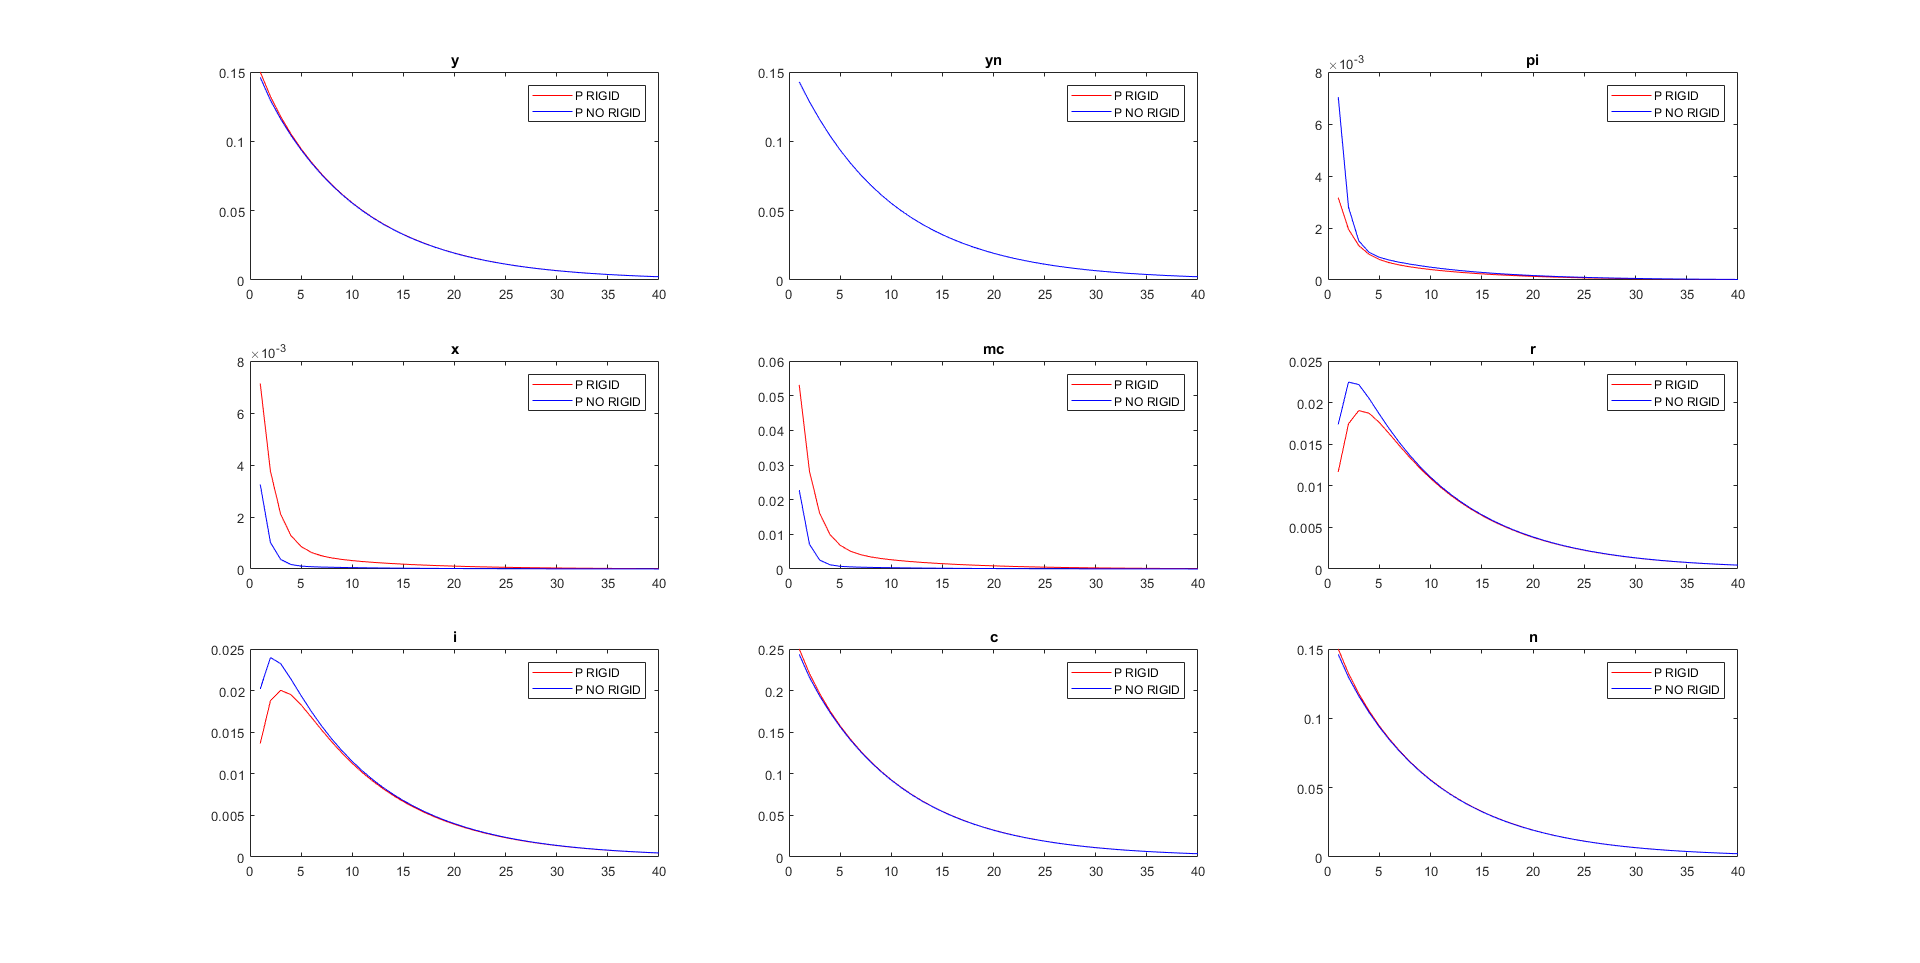
\includegraphics[scale=0.35]{./screenshots/shock_to_consumer_confidence.png}
    \label{Figure 1:}
    \caption{Shock to consumer confidence}
\end{figure}
\begin{figure}[H]
	\centering
   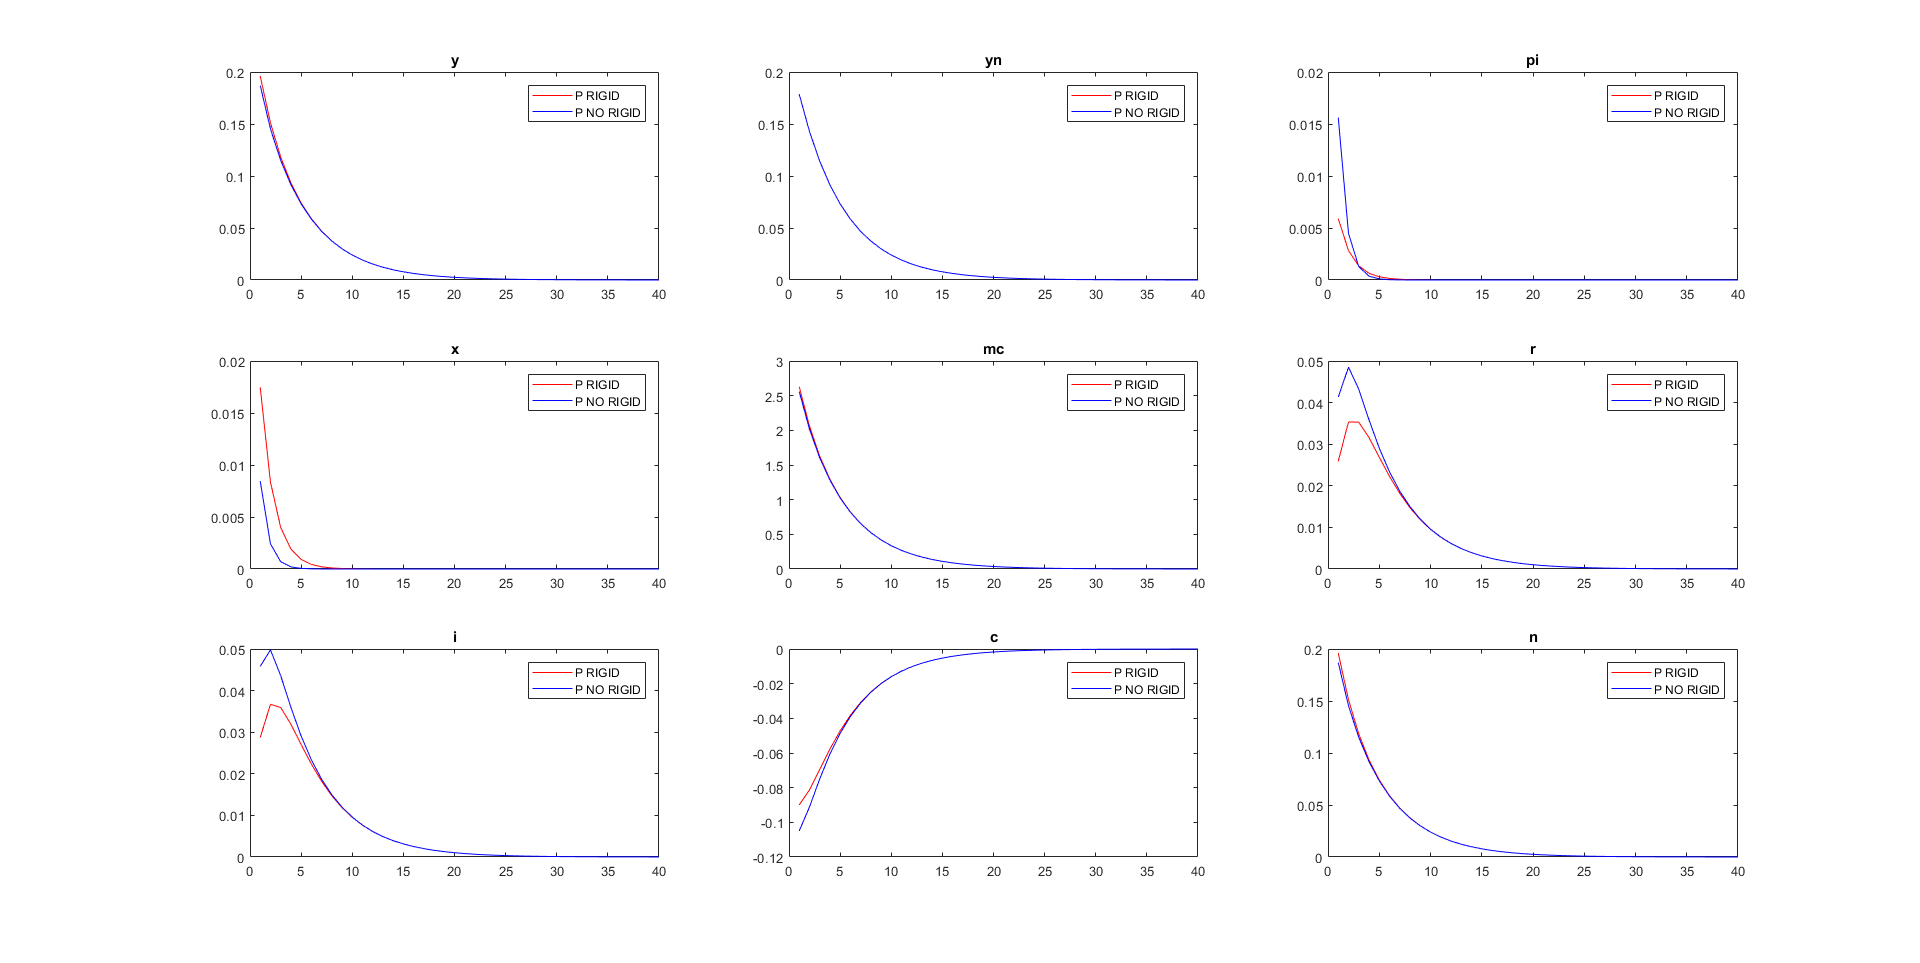
\includegraphics[scale=0.35]{./screenshots/shock_to_government_spending.png}
   \label{Figure 2:}
   \caption{Shock to government spending}
\end{figure}
\begin{figure}[H]
	\centering
   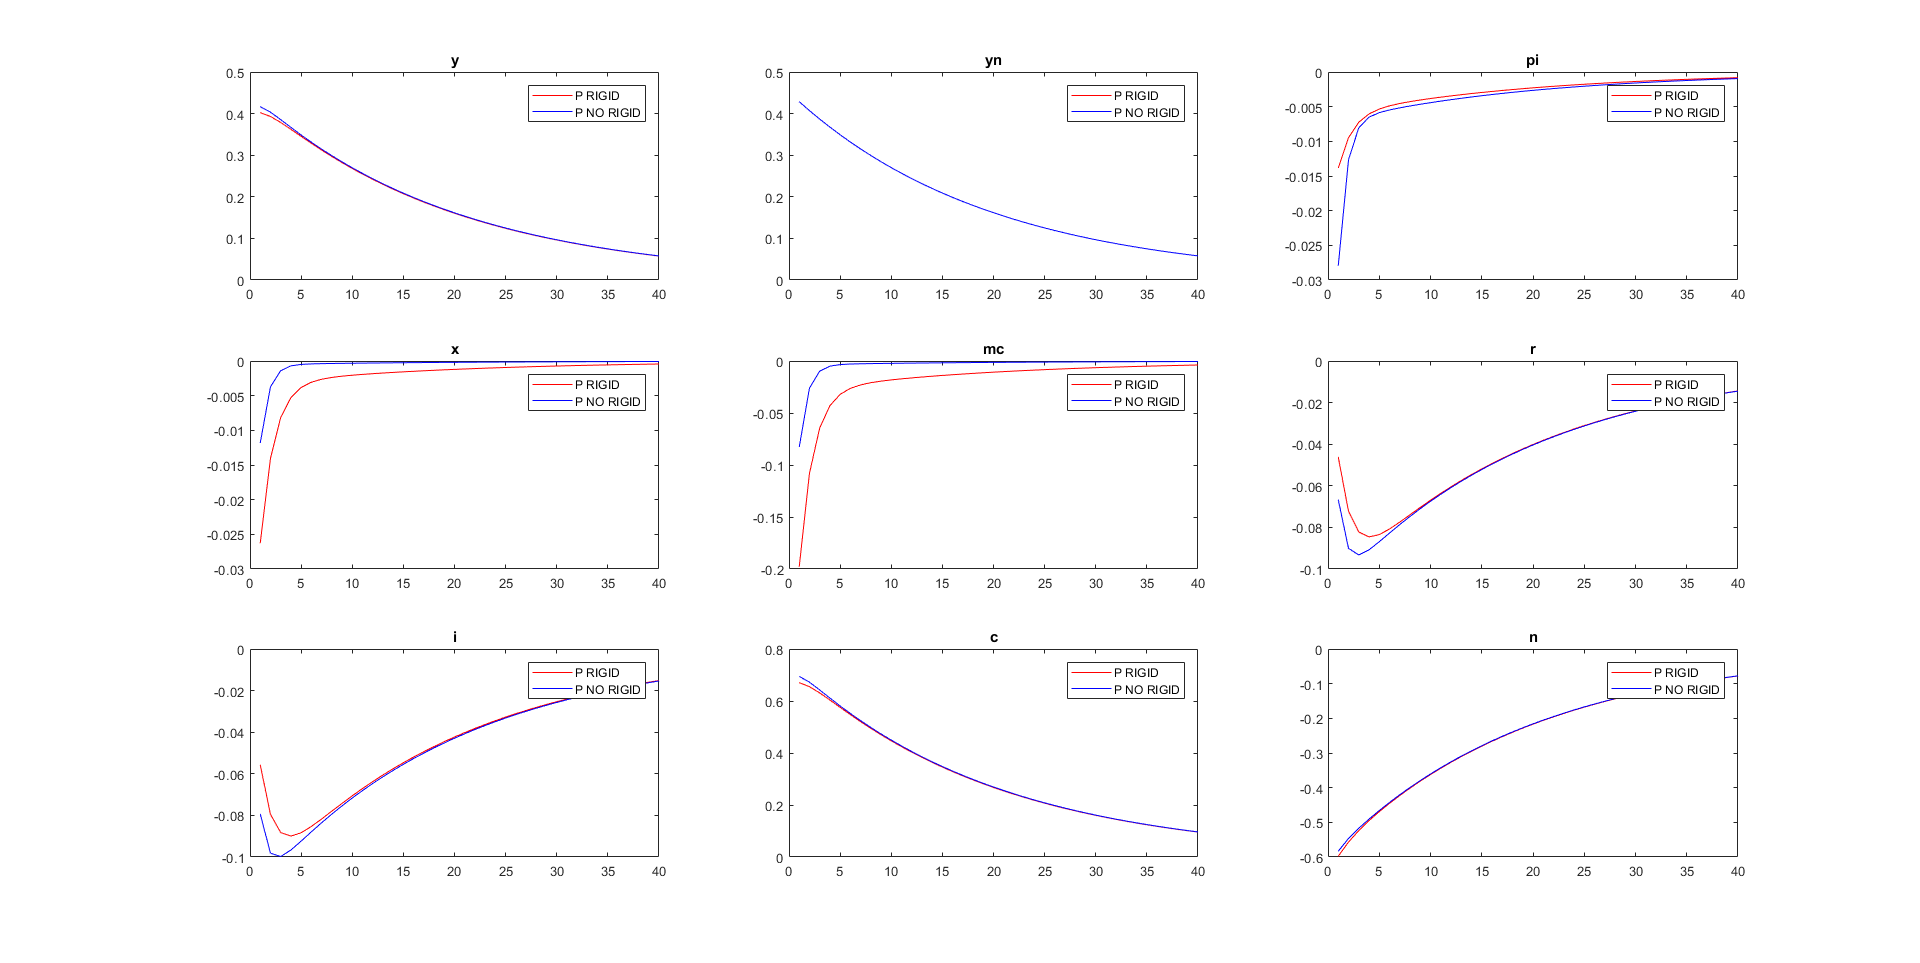
\includegraphics[scale=0.35]{./screenshots/shock_to_productivity.png}
   \label{Figure 3:}
   \caption{Shock to productivity}
\end{figure}
\begin{figure}[H]
   \centering
   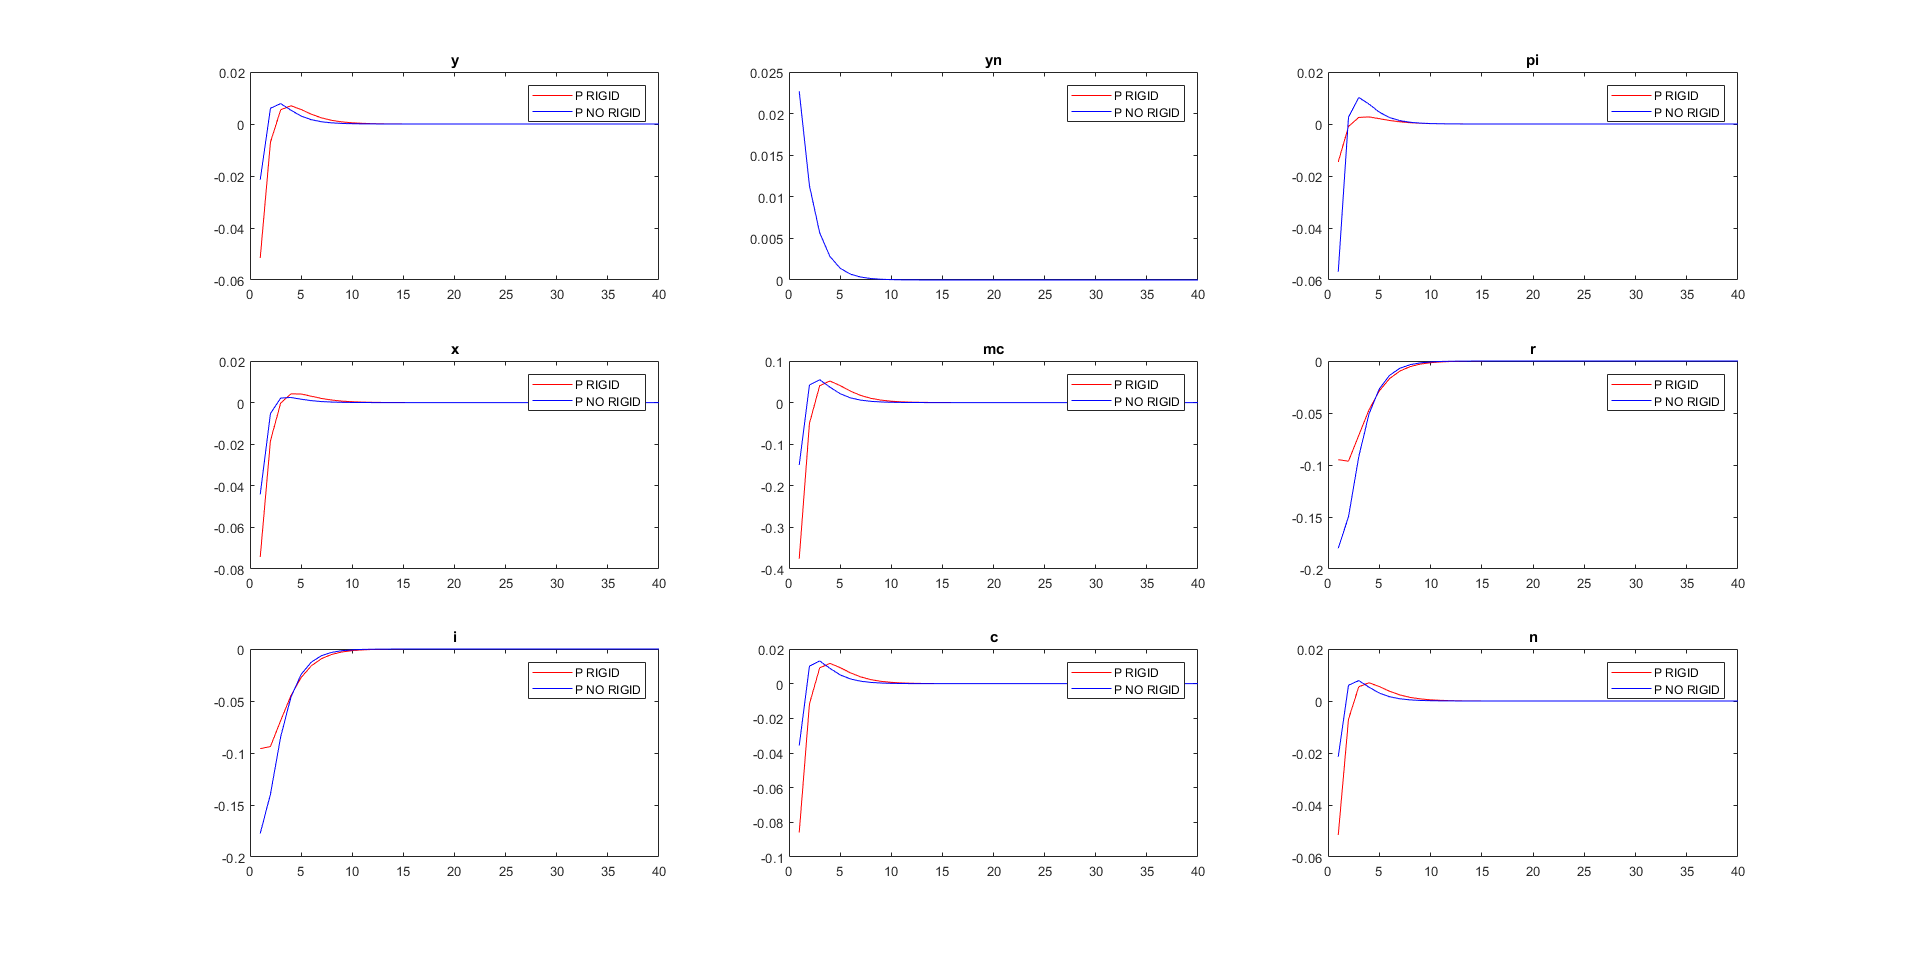
\includegraphics[scale=0.35]{./screenshots/shock_to_elasticity_of_demand.png}
   \label{Figure 4:}
   \caption{Shock to elasticity of demand}
\end{figure}
\begin{figure}[H]
	\centering
   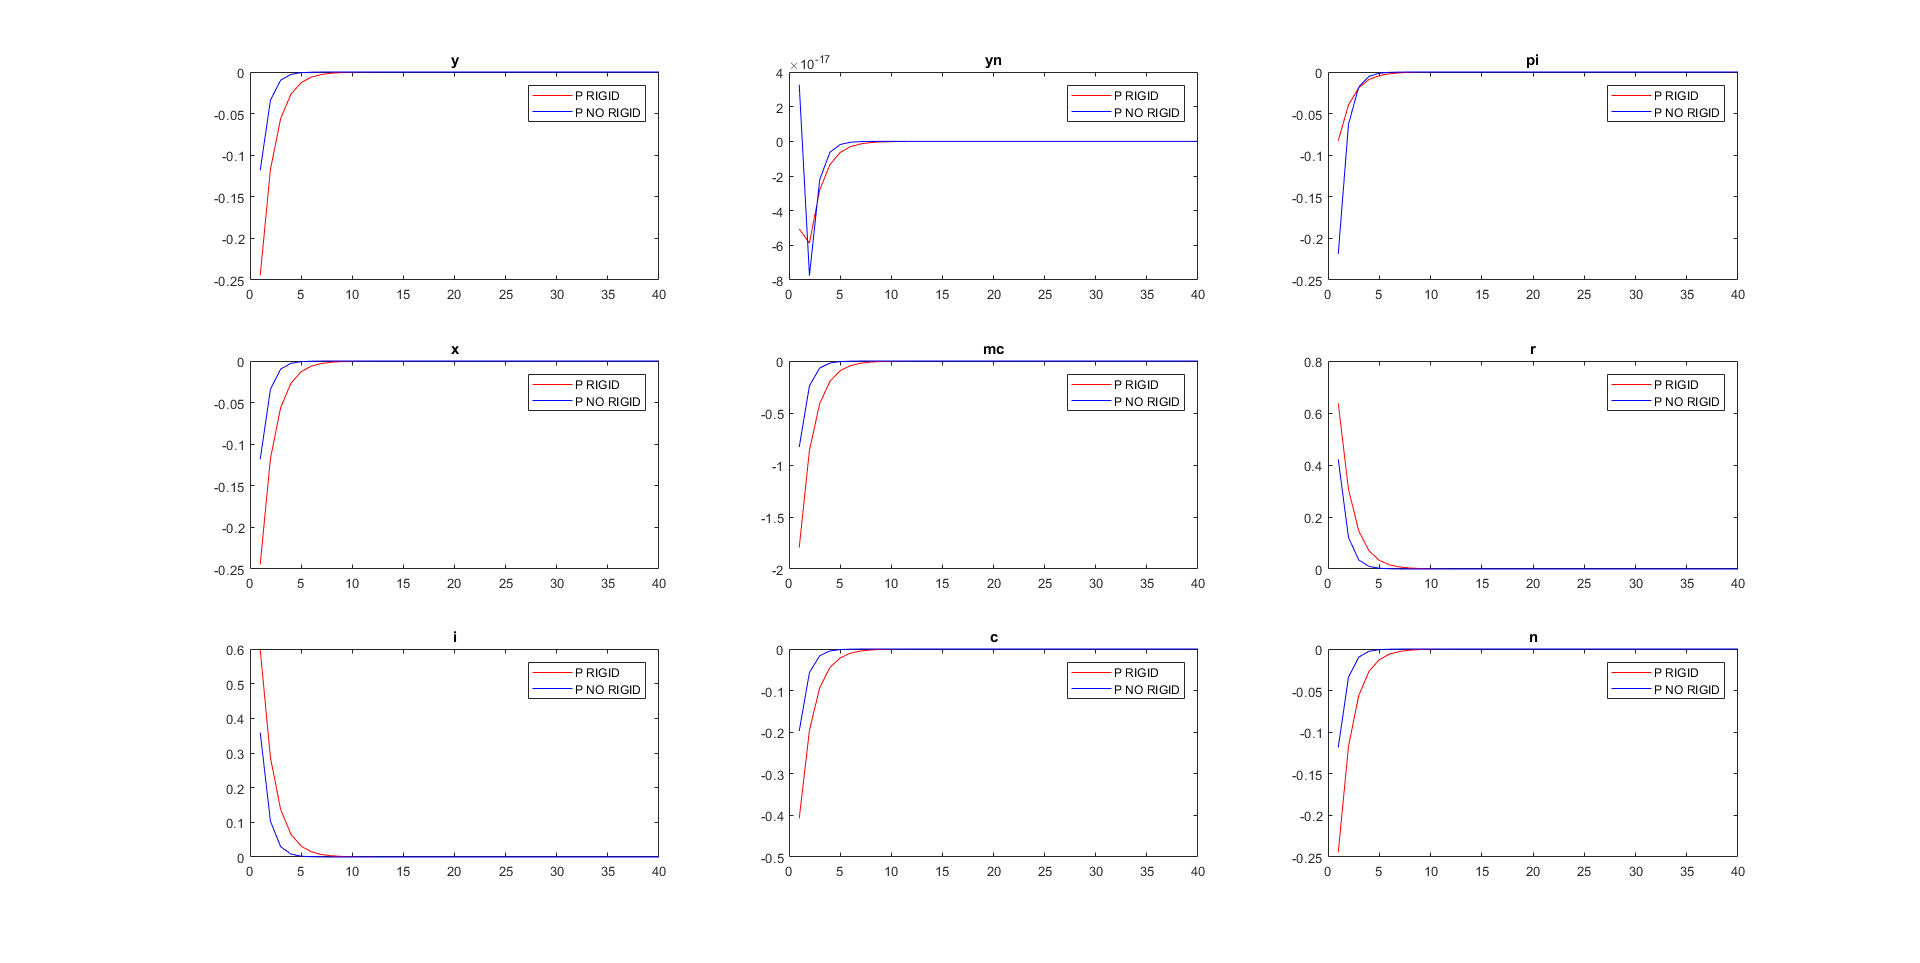
\includegraphics[scale=0.35]{./screenshots/shock_to_monetary_policy.png}
   \label{Figure 5:}
   \caption{Shock to monetary policy}
\end{figure}

The key common characteristics of the impulse response functions in the five figures above is that the reaction of inflation is much lower to all shocks when we have price rigidity in the model. Additionally, the impulse responses of the model with price rigidity are slower to adjust back to the steady state compared to the model without price rigidity. The persistence of the impulse responses is most noticeable in the inflation dynamic, output gap and marginal cost.
\end{document}
